\documentclass[12pt]{article}
\usepackage{amsmath, amssymb}
\usepackage{graphicx}
\usepackage{geometry}
\usepackage{braket}
\usepackage[authoryear]{natbib}
\usepackage{url}
\usepackage{listings}
\usepackage{subcaption}
\usepackage{booktabs}
\usepackage{multirow}
\usepackage{makecell}
\usepackage{xcolor}
\usepackage{hyperref}
\hypersetup{colorlinks=true, linkcolor=blue, citecolor=blue, urlcolor=blue}
\bibliographystyle{plainnat}
\let\cite\citep

\geometry{
  left=1.2in,
  right=1.2in,
  top=1.1in,
  bottom=1.1in
}
\usepackage{titlesec}
\usepackage{tikz}
\usetikzlibrary{arrows.meta, positioning}
\titleformat{\section}{\large\bfseries}{\thesection}{1em}{}
\titleformat{\subsection}{\normalsize\bfseries}{\thesubsection}{1em}{}
\author{Ashwot Acharya , Bishesh Bohora}
\lstset{
  basicstyle=\ttfamily\small,
  breaklines=true,
  frame=single,
  numbers=left,
  numberstyle=\tiny\color{gray},
  keywordstyle=\color{blue},
  commentstyle=\color{green!60!black},
  stringstyle=\color{red},
  showstringspaces=false
}
\title{Generalized Sudoku as a Boolean Satisfiability Problem: Comparing Native and Compact CNF encoding against Backtracking}
\date{\today}
\begin{document}
\maketitle
\begin{abstract}
Sudoku is a well-known puzzle whose generalized version can be formulated as a decision and search problem over an $n^2 \times n^2$ grid. From a computational perspective, generalized Sudoku is NP-complete, and finding a valid completion corresponds to solving a function problem in FNP. This project presents a Boolean satisfiability (SAT) based approach for solving generalized Sudoku instances by reducing the puzzle to a propositional formula in Conjunctive Normal Form (CNF).

We formally encode the structural constraints of Sudoku---definedness and uniqueness across cells, rows, columns, and sub-grids---into Boolean variables of the form $x_{i,j,k}$, representing the assignment of digit $k$ to cell $(i,j)$. The resulting constraints are translated into CNF and expressed in DIMACS format, enabling compatibility with standard SAT solvers. We adopt an optimized encoding strategy following Kwon and Jain~\cite{KwonJain2006} and compare it against a naive (full) encoding, measuring variable and clause reduction across grid sizes from $4\times4$ to $36\times36$.

The implementation generates CNF files using Python, maps logical variables to integer representations, and solves instances using the Satch SAT solver. We also compare the SAT-based method against a classical backtracking approach with MRV heuristics. A comprehensive benchmark of 75 runs across 5 grid sizes with 3 repetitions each demonstrates that SAT solving with compact encoding achieves up to 4.81$\times$ speedup over backtracking on solve-only time for $36\times36$ grids, while the compact encoding reduces variables by up to 98.7\% and clauses by up to 99.9\% compared to naive encoding. Wilcoxon signed-rank and Friedman non-parametric tests confirm statistically significant performance differences at 4 of the 5 grid sizes ($p < 0.05$). All solutions achieve a 100\% validation pass rate, verifying correctness of the SAT-based approach.
\end{abstract}
\newpage
\tableofcontents
\newpage

\section*{List of Acronyms}

\begin{tabular}{ll}
SAT   & Boolean Satisfiability Problem \\
CNF   & Conjunctive Normal Form \\
CDCL  & Conflict-Driven Clause Learning \\
DPLL  & Davis--Putnam--Logemann--Loveland Algorithm \\
DIMACS & Center for Discrete Mathematics and Theoretical Computer Science \\
MRV   & Minimum Remaining Values \\
VSIDS & Variable State Independent Decaying Sum \\
UNSAT & Unsatisfiable \\
SAT (result) & Satisfiable \\
BT    & Backtracking \\
E2E   & End-to-End \\
\end{tabular}
\newpage

\section{Introduction}
\subsection{Sudoku}
A puzzle in which an $n^2 \times n^2$ grid consisting of $n$ ``$n \times n$'' sub-grids is to be filled with numbers from $1$ to $n^2$ so that every row, column, and region contains only one instance of each number, $n \geq 1$.
In a Sudoku puzzle, some cells are already filled; these are called \textbf{clues}.
The \textbf{Sudoku Problem} is to determine whether there exists a completion such that the aforementioned conditions are satisfied.


The most common format for Sudoku is the $9  \times 9$ grid. In this project we work on larger variants. For an arbitrary positive integer $n$, we call it \textbf{Generalized Sudoku}.

\begin{figure}[h]
  \begin{minipage}{0.45\textwidth}
    \centering
  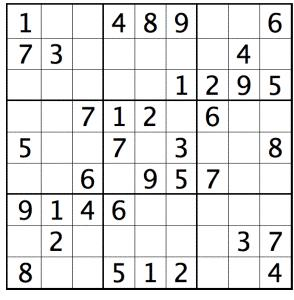
\includegraphics[width=0.8\textwidth]{graphs/unsolved.jpg}
\end{minipage}
\hfill
\begin{minipage}{0.45\textwidth}
    \centering
  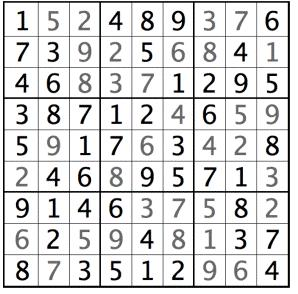
\includegraphics[width=0.8\textwidth]{graphs/solved.jpg}
\end{minipage}
  \caption{$9 \times 9 $ Sudoku and its solution  \cite{sudokueg}}
\end{figure}   

\subsubsection{Complexity of Generalized Sudoku Problem}
The Partial Latin Square Completion problem was shown to be NP-complete~\citep{Colbourn1984}. Yato and Seta~\citep{Yato2003} demonstrated that Partial Latin Square can be parsimoniously reduced to Number Place (generalized Sudoku), thereby establishing the ASP-completeness of Sudoku, which captures the computational hardness of finding another solution. Because ASP-completeness implies NP-completeness, generalized Sudoku is \textbf{NP-complete}~\citep{Yato2003}. Moreover, since the reduction in~\citep{Yato2003} is parsimonious (preserving the number of solutions), ASP-completeness also implies that counting the solutions of a generalized Sudoku instance is \#P-complete.


\subsubsection{Sudoku as CSP}
Sudoku can naturally be formulated as a Constraint Satisfaction
Problem (CSP), where each cell is a variable, the domain consists
of the numbers $\{1,\dots,n^2\}$, and the constraints enforce
row, column, and subgrid consistency.
Classical approaches solve this CSP using backtracking search
with heuristics such as Minimum Remaining Values (MRV)~\citep{RussellNorvig2010, Dechter2003}.


\subsection{The Boolean Satisfiability Problem}
In logic and computer science, the Boolean satisfiability problem (sometimes called propositional satisfiability problem and abbreviated SATISFIABILITY, SAT or B-SAT) asks whether there exists an interpretation that satisfies a given Boolean formula. In other words, it asks whether the formula's variables can be consistently replaced by the values TRUE or FALSE to make the formula evaluate to TRUE. If this is the case, the formula is called satisfiable, else unsatisfiable~\citep{wikiSAT}.\\
$ a \vee \neg b $ is SATISFIABLE with $a = 1 $ and $b = 0$.\\ 
$a \wedge \neg a $ is UNSATISFIABLE.


\subsubsection{Complexity of SAT}
SAT is NP-complete. In fact, it was the first problem to be known as such. As proved by Stephen Cook~\citep{Cook1971} at the University of Toronto in 1971 and independently by Leonid Levin at the Russian Academy of Sciences in 1973~\citep{wikiSAT}.


\subsubsection{SAT Solvers}
SAT solvers are computer programs or algorithms that check if there exist some assignment of Boolean variables in the given problem such that it evaluates to True. SAT solvers also provide the assignments. The DPLL algorithm~\citep{DPLL1962} laid the foundation for modern search-based SAT solving. Conflict-Driven Clause Learning (CDCL), introduced by GRASP~\citep{GRASP1996} and dramatically accelerated by Chaff's VSIDS decision heuristic~\citep{Chaff2001}, is now the standard architecture in solvers such as MiniSat~\citep{MiniSat2003} and the Satch solver used in this work~\citep{Satch}. CDCL combines unit propagation, conflict analysis, clause learning, and non-chronological backtracking to efficiently prune the search space. Cardinality constraints of the kind appearing in our Sudoku encoding are commonly handled with compact CNF encodings such as the sequential-counter encoding of Sinz~\citep{Sinz2005}.



\subsection{Justification for SAT approach}

Since generalized Sudoku is NP-complete (and thus belongs to NP), it can be reduced in polynomial time to any other NP-complete problem, such as Boolean satisfiability (SAT).
Note that the aforementioned complexity is for when $n$ grows without bound, but in practice we have a finite grid. 
This reduction provides a formal justification for using SAT solvers to find Sudoku solutions: by converting a Sudoku instance into an equivalent SAT instance, we can leverage modern SAT-solving algorithms to efficiently compute a valid completed grid. This approach is theoretically sound, because solving the SAT instance is guaranteed to yield a solution to the original Sudoku problem whenever one exists.
SAT solving also aids in efficient solving of CSPs~\citep{LARDEUX2020113243}.


\section{Mathematical Formulation}
\subsection{Conjunctive Normal Form}
A Boolean formula is said to be in conjunctive normal form if it is a conjunction of clauses, where each clause is a disjunction of literals~\citep{HuthRyan2004}.\\ 
The following expression is in CNF: $$( (x_1 \vee x_2) \wedge (x_2 \vee \neg x_3)  )$$\\ 
Every Boolean expression can be converted to CNF.


\subsection{Representation of Sudoku As Boolean Expression (CNF)}
Our goal is to represent the constraints of the puzzle as a Boolean expression and obtain a formula. For this we take the approach where each cell is visited and all constraints are enforced for every possible digit.


\begin{figure}[h]

\[
\renewcommand{\arraystretch}{2.5}
\begin{array}{|p{2cm}|p{2cm}||p{2cm}|p{2cm}|}
\hline
 & 2 &  &  \\
\hline
 &  & 3 &  \\
\hline\hline
 & 3  &  &  \\
\hline
 &  & 1 &  \\
\hline
\end{array}
\]
\caption{$4 \times 4$ Sudoku}
\label{fig:44}
\end{figure}


Each cell in an $n^2 \times n^2$ Sudoku has a total of $n^2$ different possible digits it can contain.
Suppose, \\
$i$:  row index  \\
$j$: column index \\ 
$k$: possible digit  \\  
$ 1 \leq i, j , k  \leq n^2$ \\ 
Then the variable $ x_{ijk} $ is true whenever the cell $(i,j)$ contains the digit $k$.


\subsubsection{Definedness}
Every cell must contain at least one digit. Every row, column and sub-grid must contain digits from 1 to $n^2$. This property is called \textbf{Definedness}.

Each cell contains at least one digit:
\[
\textbf{Cell$_d$} =
\bigwedge_{i=1}^{n^2}
\bigwedge_{j=1}^{n^2}
\left(
\bigvee_{k=1}^{n^2} x_{ijk}
\right)
\]


Each value appears at least once in each row:  
\[
\textbf{Row$_d$} =
\bigwedge_{i=1}^{n^2}
\bigwedge_{k=1}^{n^2}
\left(
\bigvee_{j=1}^{n^2} x_{ijk}
\right)
\]


Each value appears at least once in each column:  
\[
\textbf{Col$_d$} =
\bigwedge_{j=1}^{n^2}
\bigwedge_{k=1}^{n^2}
\left(
\bigvee_{i=1}^{n^2} x_{ijk}
\right)
\]

Each value appears at least once in each sub-grid:
\[
\textbf{Subgrid$_d$} =
\bigwedge_{a=0}^{n-1}
\bigwedge_{b=0}^{n-1}
\bigwedge_{k=1}^{n^2}
\left(
\bigvee_{i=1}^{n}
\bigvee_{j=1}^{n}
x_{an+i,\; bn+j,\; k}
\right)
\]


\subsubsection{Uniqueness} 

A cell can contain at most one digit and different cells in any row/column/sub-grid cannot attain the same value; these are the \textbf{Uniqueness} constraints.


Each cell contains at most one value:
\[
\textbf{Cell$_u$} =
\bigwedge_{i=1}^{n^2}
\bigwedge_{j=1}^{n^2}
\bigwedge_{1 \le k_1 < k_2 \le n^2}
(\neg x_{i,j,k_1} \lor \neg x_{i,j,k_2})
\]

Each value appears at most once in every row:
\[
\textbf{Row$_u$} =
\bigwedge_{i=1}^{n^2}
\bigwedge_{k=1}^{n^2}
\bigwedge_{1 \le j_1 < j_2 \le n^2}
(\neg x_{i,j_1,k} \lor \neg x_{i,j_2,k})
\]

Each value appears at most once in every column:
\[
\textbf{Col$_u$} =
\bigwedge_{j=1}^{n^2}
\bigwedge_{k=1}^{n^2}
\bigwedge_{1 \le i_1 < i_2 \le n^2}
(\neg x_{i_1,j,k} \lor \neg x_{i_2,j,k})
\]

Each value appears at most once in every subgrid:
\[
\textbf{Subgrid$_u$} =
\bigwedge_{a=0}^{n-1}
\bigwedge_{b=0}^{n-1}
\bigwedge_{k=1}^{n^2}
\bigwedge_{\substack{(i_1,j_1),(i_2,j_2) \\ 1 \le i_1,j_1,i_2,j_2 \le n \\ i_1 < i_2, j_1<j_2}}
(\neg x_{an+i_1,\; bn+j_1,\; k}
 \lor
 \neg x_{an+i_2,\; bn+j_2,\; k})
\]

\subsubsection*{For Clues}

If the puzzle contains a fixed entry $(i,j)=k$, it is encoded as a unit clause:
\[
\textbf{Clues} =
\bigwedge_{(i,j,k)\in G} x_{i,j,k}
\]
which forces them to be true.



\subsubsection*{Example}

For the given $4 \times 4$ Sudoku in Figure~\ref{fig:44}, we introduce Boolean variables
\[
x_{i,j,k}
\]
with $i,j,k \in \{1,2,3,4\}$, where
\[
x_{i,j,k} = 1 \quad \text{iff cell } (i,j) \text{ contains number } k.
\]

Thus, we obtain $4^3 = 64$ Boolean variables.


Each cell must contain at least one number:
\[
\bigvee_{k=1}^{4} x_{i,j,k}
\quad \text{for all } i,j.
\]

For cell $(1,1)$:
\[
x_{1,1,1} \lor x_{1,1,2} \lor x_{1,1,3} \lor x_{1,1,4}.
\]

Each cell contains at most one number:
\[
\neg x_{i,j,k} \lor \neg x_{i,j,\ell}
\quad \text{for all } k \neq \ell.
\]

\[
\neg x_{1,1,1} \lor \neg x_{1,1,2}.
\]


Each number appears exactly once in every row.

At least once:
\[
\bigvee_{j=1}^{4} x_{i,j,k}
\quad \text{for all } i,k.
\]

For number 1 in row 1:
\[
x_{1,1,1} \lor x_{1,2,1} \lor x_{1,3,1} \lor x_{1,4,1}.
\]

At most once:
\[
\neg x_{i,j,k} \lor \neg x_{i,\ell,k}
\quad \text{for } j \neq \ell.
\]


Each number appears exactly once in every column.

At least once:
\[
\bigvee_{i=1}^{4} x_{i,j,k}
\quad \text{for all } j,k.
\]

For number 2 in column 2:
\[
x_{1,2,2} \lor x_{2,2,2} \lor x_{3,2,2} \lor x_{4,2,2}.
\]

At most once:
\[
\neg x_{i,j,k} \lor \neg x_{\ell,j,k}
\quad \text{for } i \neq \ell.
\]


Each number appears exactly once in every $2 \times 2$ subgrid.

For example, in the upper-left block (rows 1--2, columns 1--2):

At least once (number 1):
\[
x_{1,1,1} \lor x_{1,2,1} \lor x_{2,1,1} \lor x_{2,2,1}.
\]

At most once:
\[
\neg x_{1,1,1} \lor \neg x_{2,2,1},
\]
and similarly for all other pairs.

\subsection*{Encoding the Given Puzzle}

The fixed entries of the puzzle are encoded as unit clauses.

From the grid:
\[
(1,2)=2 \quad \Rightarrow \quad x_{1,2,2}
\]
\[
(2,3)=3 \quad \Rightarrow \quad x_{2,3,3}
\]
\[
(3,2)=3 \quad \Rightarrow \quad x_{3,2,3}
\]
\[
(4,3)=1 \quad \Rightarrow \quad x_{4,3,1}
\]

Each of these is added as a unit clause to the CNF formula.


\subsubsection{Final Formula}
We present the reduced CNF formula $\phi'$ of Kwon and Jain~\citep{KwonJain2006}, which reflects the given clues by eliminating variables and clauses that are already satisfied. It builds on the extended encoding of Lynce and Ouaknine~\citep{SuSAT}. The complete CNF encoding is:
\[
\phi = \text{Clues} \Downarrow V^{+}
\;\cup\;
\left( \text{Cell}_{u} \cup \text{Row}_{u} \cup \text{Col}_{u} \cup \text{Subgrid}_{u} \right) \Downarrow V^{-}
\;\cup\;
\left( \text{Cell}_{d} \cup \text{Row}_{d} \cup \text{Col}_{d} \cup \text{Subgrid}_{d} \right) \downarrow V^{-}
\]

where:\\
$V^+ = \text{Set of variables with true assignment}$\\
$V^- = \text{Set of variables with false assignments}$\\ 
$\Downarrow \text{eliminates clauses that are satisfied}$ \\
$\downarrow \text{eliminates literals that are falsified}$\\
Note that each constraint here is treated as a set of clauses; the formula is in CNF.


\section{Implementation}

\subsection{Computer Representation}

The Sudoku puzzle is first represented in a plain text file. 
With the decided encoding, the problem is converted to CNF using the \textbf{DIMACS} format.
\subsubsection{DIMACS Format}
It is a textual representation of a formula in CNF form, where each line ending with 0 represents a clause. Each literal and its negation is represented by a positive and negative integer respectively.
A DIMACS CNF file starts with a header \texttt{p cnf (variables) (clauses)} where \texttt{(variables)} and \texttt{(clauses)} are replaced with the number of variables and clauses respectively. Any line beginning with \texttt{c} is a comment.
The formula $( x \vee y \vee \neg z ) \land (\neg x \vee \neg y )$ in DIMACS format would be 
\begin{verbatim}
  p cnf 3 2
  1 2 3 0
  -1 -2 0
\end{verbatim}
where variables $x,y,z$ are represented by $1,2,3$.


\subsection{Mapping variables to integers}
To obtain valid DIMACS format each triplet $(i,j,k)$, $1\leq i, j, k \leq n^2$ is mapped to a positive integer:
\[
V(i, j, k) = (i - 1)n^4 + (j - 1)n^2 + k
\]

Given a DIMACS variable number $V$, the inverse mapping recovers $(i,j,k)$:
\[
i = \left\lfloor \frac{V-1}{n^{4}} \right\rfloor + 1
\]
\[
j = \left\lfloor \frac{(V-1) \bmod n^{4}}{n^{2}} \right\rfloor + 1
\]
\[
k = \big((V-1) \bmod n^{2}\big) + 1
\]

\begin{quote}
\emph{Notation remark.} In the mathematical formulation above, $n$ denotes the size of a box, so the whole grid is $n^2 \times n^2$ (e.g., a $36\times36$ grid has $n=6$). In the code listings in the Appendix, by contrast, $n$ denotes the full grid size and $\texttt{box} = \lfloor\sqrt{n}\rfloor$ is used for the box width (e.g., grid $n=36$, box $=6$).
\end{quote}


\subsection{Solution Using SAT Solvers}

We use {\tt Satch} (Armin Biere's {\tt SATCH} v0.5.6rc \citep{Satch}) as our primary SAT solver. The generated clauses are written to DIMACS format and passed to Satch. If the formula is satisfiable, the solver returns a model, which is decoded using the inverse mapping to reconstruct the completed Sudoku grid.


\subsection{Dual CNF Encoding}
\label{sec:encoding}

We implement and compare two CNF encoding strategies for Sudoku~\citep{KwonJain2006}:

\subsubsection{Naive (Full) Encoding $\phi$}
Uses the full $n^3$ variable space with no optimization from given clues. Each possible $(r,c,v)$ triple maps to a Boolean variable regardless of whether the cell is pre-filled. This produces $\mathcal{O}(n^6)$ clauses.

\subsubsection{Compact Encoding $\phi'$}
Follows the optimized encoding of Kwon and Jain~\citep{KwonJain2006}. Given clues are substituted directly: if cell $(r,c)$ is filled with value $v$, variables $x_{r,c,v'}$ for $v' \neq v$ are set to false, and peer variables involving value $v$ in the same row, column, and block are eliminated. This produces significantly fewer variables and clauses, especially for puzzles with many clues.

The variable counts are:
\begin{itemize}
    \item Naive: $n^3$ variables (e.g., 46{,}656 for $36\times36$)
    \item Compact: only free (undetermined) variables remain (e.g., $\sim$600 for $36\times36$)
\end{itemize}


\section{Experimental Setup}

\subsection{Dataset}
The benchmark dataset consists of 25 puzzles across 5 grid sizes, generated with seed-controlled reproducibility:

\begin{itemize}
    \item \textbf{4$\times$4}: 5 hand-constructed puzzles (4--6 clues each)
    \item \textbf{9$\times$9}: 5 puzzles from Gordon Royle's 17-clue database (proven unique solutions)
    \item \textbf{16$\times$16, 25$\times$25, 36$\times$36}: Procedurally generated via solution construction with cell removal, verified through constraint propagation
\end{itemize}

The clue counts of the sampled runs were $\{6,4,4,4,4\}$ for $4\times4$ (25--38\% of cells), $\{17,17,17,17,16\}$ for the $9\times9$ group (the Royle collection is a 17-clue database but one sampled puzzle retained only 16 clues), and $\{161,181,201,141,151\}$, $\{381,411,381,351,381\}$, and $\{1041,931,1041,951,991\}$ for $16\times16$, $25\times25$, and $36\times36$, corresponding to densities of 55--79\%, 56--66\%, and 72--80\%, respectively. Because the compact encoding prunes variables in cells or values forced by given clues, this high clue density for $n \geq 16$ is the regime where the variable and clause reductions of Section~\ref{sec:encoding} are most pronounced. Independent results support the difficulty of sparse large grids: McGuire, Tugemann, and Civario~\citep{McGuire2014} proved that every solvable $9\times9$ Sudoku has at least 17 clues, and Eppstein and Zhang~\citep{EppsteinZhang2026} showed that for large $n$, almost every $n^2\times n^2$ grid requires $n^4 - O(n^4/\log n)$ clues (only a logarithmic fraction of cells can be unfilled), so the dense clue distributions used here reflect genuinely typical instances.

\subsection{Benchmark Protocol}
Each puzzle is solved by three methods:
\begin{enumerate}
    \item \textbf{SAT Compact}: Encoded with $\phi'$ (Kwon and Jain optimization) and solved by Satch
    \item \textbf{SAT Naive}: Encoded with $\phi$ (full encoding) and solved by Satch
    \item \textbf{Backtracking (BT)}: Classical backtracking with MRV heuristic and forward checking
\end{enumerate}

\noindent Each solution is run 3 times (repetitions) for a total of 75 benchmark runs. A 600-second timeout is enforced. All returned solutions are validated post-hoc against the puzzle constraints.

All experiments ran on a single machine (AMD Ryzen 5 7235HS, 8 cores, 16\,GB RAM, Linux 6.18.45-1-MANJARO x86-64) using Python 3 and the Satch~\citep{Satch} solver. No run in this dataset reached the timeout; timeout handling is retained for robustness and is reported explicitly where it occurs.

\subsection{Metrics}
We report:
\begin{itemize}
    \item \textbf{Solve-only time}: Time spent in the solver (SAT or BT), excluding encoding
    \item \textbf{End-to-end (E2E) time}: Encoding time + solve time
    \item \textbf{CNF size}: Number of variables and clauses
    \item \textbf{Validation pass rate}: Fraction of solutions passing constraint validation
\end{itemize}


\section{Results}

\subsection{Solver Performance (Solve-Only Time)}

Table~\ref{tab:solve_only} reports the mean solve-only time for each solver across grid sizes. Timeout runs are reported separately; upper-bound means treat each timeout as 600\,s.

\begin{table}[htbp]
\centering
\caption{Solver performance: solve-only time (mean $\pm$ std).}
\label{tab:solve_only}
\resizebox{\textwidth}{!}{%
\begin{tabular}{lccccc}
\toprule
\textbf{Size} & \textbf{SAT Compact} & \textbf{SAT Naive} & \textbf{Backtracking} & \textbf{Speedup BT/SAT-C} & \textbf{Speedup N/C} \\
\midrule
4$\times$4    & 0.001s$\pm$0.24ms  & 0.001s$\pm$0.23ms  & 0.05ms$\pm$0.01ms    & 0.04$\times$ & 0.94$\times$ \\
9$\times$9    & 0.002s$\pm$0.27ms  & 0.003s$\pm$0.23ms  & 0.003s$\pm$0.004s    & 1.71$\times$ & 1.33$\times$ \\
16$\times$16  & 0.002s$\pm$0.21ms  & 0.013s$\pm$0.64ms  & 0.95ms$\pm$0.37ms    & 0.59$\times$ & 8.38$\times$ \\
25$\times$25  & 0.002s$\pm$0.42ms  & 0.078s$\pm$0.004s  & 0.010s$\pm$0.007s    & 4.04$\times$ & 31.95$\times$ \\
36$\times$36  & 0.002s$\pm$0.002s  & 0.347s$\pm$0.011s  & 0.012s$\pm$0.003s    & 4.81$\times$ & 144.33$\times$ \\
\bottomrule
\end{tabular}}
\vspace{0.5ex}

\begin{flushleft}
{\small Speedup values $<1$ mean the first-named solver is {\em faster}: e.g., ``0.04$\times$'' at $4\times4$ indicates backtracking is $\sim$20$\times$ faster than SAT Compact in solve-only time, and ``0.94$\times$'' indicates the naive encoding is marginally faster at $4\times4$.}
\end{flushleft}
\end{table}

Key observations:
\begin{itemize}
    \item \textbf{SAT Compact} maintains near-constant solve time ($\sim$2\,ms) across all grid sizes, demonstrating the power of the compact encoding combined with CDCL propagation.
    \item \textbf{SAT Naive} solve time grows with grid size due to the larger search space ($n^3$ variables).
    \item \textbf{Backtracking} wins in solve-only time at $4\times4$ and $16\times16$ but is overtaken by SAT Compact at $25\times25$, becoming $\sim$4.8$\times$ slower at $36\times36$.
    \item The \textbf{Naive/Compact speedup} reaches 144$\times$ at $36\times36$, demonstrating the dramatic effect of encoding optimization on SAT solver performance.
\end{itemize}


\subsection{End-to-End Performance (Encoding + Solve)}

Table~\ref{tab:e2e} reports the end-to-end time including CNF encoding overhead.

\begin{table}[htbp]
\centering
\caption{End-to-end performance: encoding + solve time.}
\label{tab:e2e}
\resizebox{\textwidth}{!}{%
\begin{tabular}{lccccc}
\toprule
\textbf{Size} & \textbf{Compact Enc} & \textbf{Naive Enc} & \textbf{SAT-C E2E} & \textbf{SAT-N E2E} & \textbf{BT} \\
\midrule
4$\times$4    & 0.32ms   & 0.16ms   & 0.001s   & 0.001s   & 0.05ms \\
9$\times$9    & 0.007s   & 0.004s   & 0.009s   & 0.007s   & 0.003s \\
16$\times$16  & 0.043s   & 0.047s   & 0.044s   & 0.061s   & 0.95ms \\
25$\times$25  & 0.246s   & 0.512s   & 0.248s   & 0.590s   & 0.010s \\
36$\times$36  & 1.046s   & 1.911s   & 1.048s   & 2.258s   & 0.012s \\
\bottomrule
\end{tabular}}
\end{table}

The E2E perspective reveals that:
\begin{itemize}
    \item \textbf{CNF encoding is the dominant cost} for SAT solving. For $36\times36$, encoding takes 1.05\,s (compact) or 1.91\,s (naive), while solving takes $<$10\,ms.
    \item The \textbf{compact encoding reduces E2E time by 53\%} compared to naive at $36\times36$ (1.05\,s vs.\ 2.26\,s).
    \item Backtracking remains fastest in E2E for these puzzle densities because it requires no encoding step.
\end{itemize}


\subsection{CNF Dual Encoding Comparison}

Table~\ref{tab:encoding} compares the naive and compact encoding sizes.

\begin{table}[htbp]
\centering
\caption{CNF encoding size comparison: naive ($\phi$) vs.\ compact ($\phi'$).}
\label{tab:encoding}
\resizebox{\textwidth}{!}{%
\begin{tabular}{lrrrrrr}
\toprule
\textbf{Size} & \textbf{Naive Vars} & \textbf{Naive Clauses} & \textbf{Compact Vars} & \textbf{Compact Clauses} & \textbf{Var Red.} & \textbf{Clause Red.} \\
\midrule
4$\times$4    & 64       & 452           & 21  & 96      & 66.2\%  & 78.8\%  \\
9$\times$9    & 729      & 12{,}004      & 318 & 3{,}113 & 56.3\%  & 74.1\%  \\
16$\times$16  & 4{,}096  & 124{,}071     & 197 & 1{,}085 & 95.2\%  & 99.1\%  \\
25$\times$25  & 15{,}625 & 752{,}881     & 780 & 5{,}731 & 95.0\%  & 99.2\%  \\
36$\times$36  & 46{,}656 & 3{,}272{,}095 & 607 & 3{,}194 & 98.7\%  & 99.9\%  \\
\bottomrule
\end{tabular}}
\end{table}

The compact encoding achieves dramatic reductions:
\begin{itemize}
    \item For $36\times36$: \textbf{98.7\% variable reduction} (46{,}656 $\to$ 607) and \textbf{99.9\% clause reduction} (3{,}272{,}095 $\to$ 3{,}194)
    \item Reductions increase with grid size, demonstrating that the optimization exploits clue structure more effectively on larger puzzles
\end{itemize}


\subsection{Scaling Visualization}

Figure~\ref{fig:scaling} shows the scaling behavior across all grid sizes on a log scale.

\begin{figure}[htbp]
\centering

\includegraphics[width=0.85\textwidth]{graphs/plot_scaling.png}
\caption{Mean solve time (log scale) across grid sizes for SAT Compact, SAT Naive, and Backtracking solvers.}
\label{fig:scaling}
\end{figure}

Figure~\ref{fig:speedup} shows the speedup ratios.

\begin{figure}[htbp]
\centering

\includegraphics[width=0.85\textwidth]{graphs/plot_speedup.png}
\caption{Speedup ratios: BT/SAT Compact and SAT Naive/SAT Compact across grid sizes.}
\label{fig:speedup}
\end{figure}

Figure~\ref{fig:overview} provides a comprehensive view of all solver times.

\begin{figure}[htbp]
\centering

\includegraphics[width=0.85\textwidth]{graphs/plot_overview.png}
\caption{Overview of all solver times across grid sizes.}
\label{fig:overview}
\end{figure}

Figure~\ref{fig:cnf_encoding} compares the encoding sizes visually.

\begin{figure}[htbp]
\centering
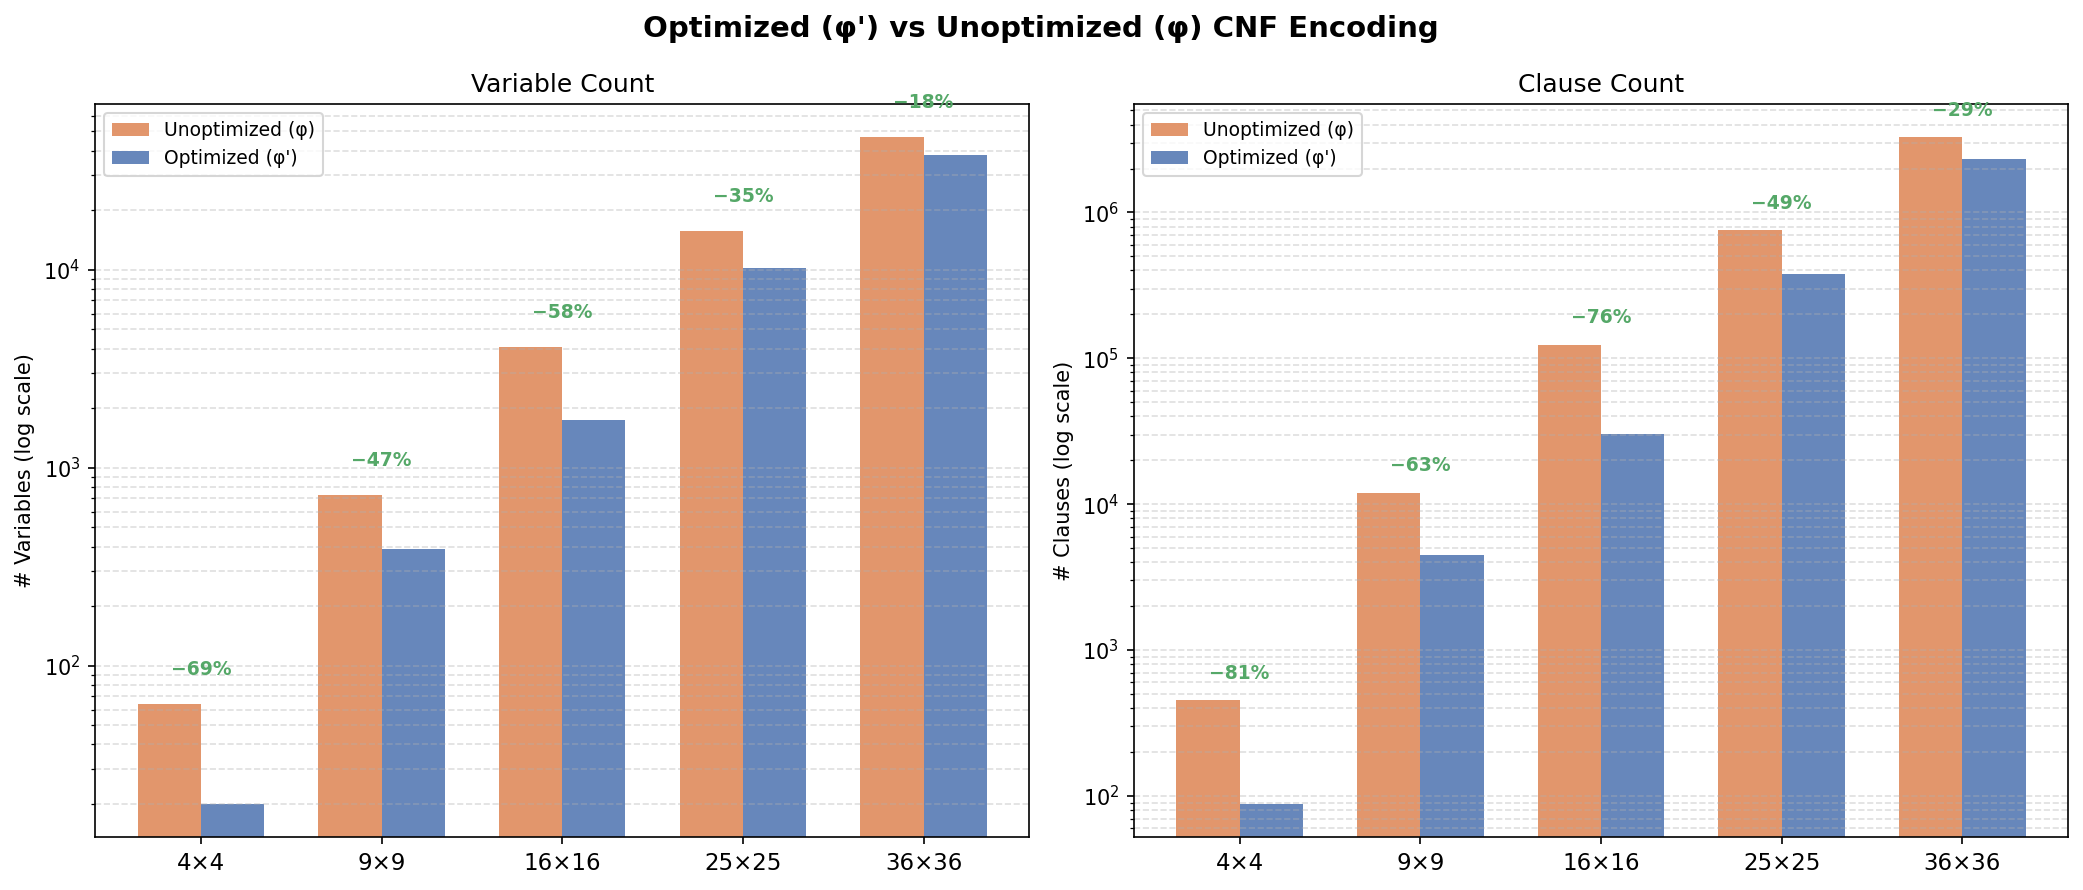
\includegraphics[width=0.85\textwidth]{graphs/cnf_encoding_comparison.png}
\caption{Naive vs.\ compact encoding: variable and clause counts across grid sizes.}
\label{fig:cnf_encoding}
\end{figure}


\section{Statistical Analysis}

\subsection{Methodology}

We employ non-parametric statistical tests to rigorously compare solver performance. Non-parametric tests are appropriate here because:
\begin{itemize}
    \item Timing distributions are heavily right-skewed, with a 600\,s timeout used to censor pathologically slow runs (none occurred in this dataset)
    \item Sample sizes are modest ($n = 15$ per group)
    \item No assumption of normality is warranted
\end{itemize}

We apply the Wilcoxon signed-rank test~\citep{Wilcoxon1945} for paired pairwise comparisons and the Friedman test~\citep{Friedman1937} with Kendall's $W$~\citep{Kendall1948} for omnibus multi-solver comparison. All tests use $\alpha = 0.05$.


\subsection{Wilcoxon Signed-Rank Test: BT vs.\ SAT Compact}

The Wilcoxon signed-rank test is a non-parametric paired test that evaluates whether the median difference between two related samples differs from zero. We compare backtracking and SAT Compact solve times for each puzzle (paired by puzzle and repetition).

\begin{table}[htbp]
\centering
\caption{Wilcoxon signed-rank test: BT vs.\ SAT Compact solve time.}
\label{tab:wilcoxon}
\begin{tabular}{lccccc}
\toprule
\textbf{Size} & \textbf{N pairs} & \textbf{W} & \textbf{p-value} & \textbf{Significant} & \textbf{Mean BT / SAT-C} \\
\midrule
4$\times$4    & 15 & 0.00  & $<$0.001 & \textcolor{red}{Yes} & 0.05ms / 0.001s \\
9$\times$9    & 15 & 45.00 & 0.421   & No & 0.003s / 0.002s \\
16$\times$16  & 15 & 1.00  & $<$0.001 & \textcolor{red}{Yes} & 0.95ms / 0.002s \\
25$\times$25  & 15 & 0.00  & $<$0.001 & \textcolor{red}{Yes} & 0.010s / 0.002s \\
36$\times$36  & 15 & 0.00  & $<$0.001 & \textcolor{red}{Yes} & 0.012s / 0.002s \\
\bottomrule
\end{tabular}
\end{table}

The Wilcoxon test reveals statistically significant differences at 4 out of 5 grid sizes ($p < 0.001$). At $9\times9$, the difference is not significant ($p = 0.421$), indicating that for minimal-clue 17-clue puzzles, both solvers perform comparably. The sign of the detected difference is size-dependent: at $4\times4$ and $16\times16$ backtracking is significantly \emph{faster} in solve-only time, whereas at $25\times25$ and $36\times36$ SAT Compact is significantly faster.


\subsection{Friedman Test: Multi-Solver Comparison}

The Friedman test evaluates whether there are significant differences among all three solvers simultaneously, treating each puzzle as a block (repeated measure).

\begin{table}[htbp]
\centering
\caption{Friedman test (BT vs.\ SAT-C vs.\ SAT-N) with Kendall's $W$ effect size.}
\label{tab:friedman}
\begin{tabular}{lccccc}
\toprule
\textbf{Size} & \textbf{N blocks} & \textbf{$\chi^2$} & \textbf{p-value} & \textbf{Kendall's $W$} & \textbf{Significant} \\
\midrule
4$\times$4    & 5 & 7.60  & 0.022 & 0.760 & \textcolor{red}{Yes} \\
9$\times$9    & 5 & 2.80  & 0.247 & 0.280 & No \\
16$\times$16  & 5 & 10.00 & 0.007 & 1.000 & \textcolor{red}{Yes} \\
25$\times$25  & 5 & 10.00 & 0.007 & 1.000 & \textcolor{red}{Yes} \\
36$\times$36  & 5 & 10.00 & 0.007 & 1.000 & \textcolor{red}{Yes} \\
\bottomrule
\end{tabular}
\end{table}

Key findings from the inferential analysis:
\begin{itemize}
    \item \textbf{Statistically significant differences exist at 4 of 5 sizes} ($p < 0.05$), confirming that solver choice matters.
    \item \textbf{Kendall's $W = 1.0$} at $16\times16$ through $36\times36$ indicates \emph{perfect agreement} among blocks within each size: every puzzle at that size induces the same ranking of the three solvers (backtracking $<$ SAT Compact $<$ SAT Naive at $16\times16$; SAT Compact $<$ backtracking $<$ SAT Naive at $25\times25$ and $36\times36$).
    \item At $9\times9$ (17-clue minimal puzzles), all solvers perform similarly ($p = 0.247$), consistent with the puzzle being well-constrained.
    \item At $4\times4$, the significant difference ($W = 0.76$) reflects backtracking being far faster in solve-only time on trivial instances: the SAT solver's fixed startup cost dominates at this scale.
\end{itemize}


\subsection{Solution Correctness}

All 75 benchmark runs achieve a 100\% validation pass rate. Every solution returned by every solver passes row, column, and sub-grid constraint validation. Pre-generation uniqueness is verified through constraint propagation and SAT-based blocking where applicable. This confluence is consistent with Mašulović's result~\citep{Masulovic2022} that a Sudoku grid's solution is unique if and only if it can be logically deduced in the propagation-based ``Sudoku logic'', which underpins our use of propagation-driven uniqueness checking.


\section{Discussion}

\subsection{Encoding Optimization is Critical}
The compact encoding reduces the CNF formula by over 99\% for large grids, and this reduction directly translates to faster SAT solve times. Without it, the naive encoding's $n^3$ variables create an unnecessarily large search space that degrades CDCL performance.

\subsection{SAT vs.\ Backtracking: A Size-Dependent Trade-off}
For small puzzles ($4\times4$), backtracking is marginally faster because it avoids encoding overhead. For large puzzles ($\geq 25\times25$), SAT Compact dominates due to efficient unit propagation and clause learning. The crossover occurs around $9\times9$ to $16\times16$.

\subsection{Encoding Time Dominates E2E}
The end-to-end analysis reveals that for puzzles up to $36\times36$, the SAT solve time is negligible ($<$10\,ms) while encoding takes up to 2\,s. This suggests that for practical Sudoku solving, encoding optimization should be the primary focus.

\subsection{Statistical Rigor}
The use of non-parametric tests (Wilcoxon, Friedman) provides statistically rigorous evidence for the observed performance differences, addressing concerns about the validity of timing-based benchmarks with small sample sizes.

\subsection{Limitations}
Several caveats should be kept in mind. First, the SAT results reflect a single solver (Satch~\citep{Satch}); a modern CDCL baseline such as MiniSat or Glucose was not benchmarked, and the custom C CDCL core in Appendix~\ref{app:cdcl} is a standalone study component that is not part of the reported timings. Second, the 5-puzzle $\times$ 3-repetition design gives substantial within-size power for paired tests but only $n=5$ independent puzzles per size, so omnibus (Friedman) results at each size rest on a small number of blocks. Third, all production grids of size $n \geq 16$ are clue-dense (55--80\% of cells fixed), which is the regime where the compact encoding's clue-based pruning is strongest and where SAT is most competitive; sparse large grids, which Eppstein and Zhang~\citep{EppsteinZhang2026} argue are increasingly rare as $n$ grows, may favor a different comparison. Finally, the solve-only advantage of 4.81$\times$ at $36\times36$ is computed on sub-10\,ms solve times; end-to-end, backtracking remains fastest overall because SAT must pay a 1--2\,s encoding cost.


\section{Conclusion}

This project investigated the use of Boolean satisfiability (SAT) solving as an approach to solving Sudoku puzzles by encoding the problem as a formula in conjunctive normal form (CNF). The Sudoku constraints were translated into logical clauses, and solutions were obtained using the Satch SAT solver with two encoding strategies.

The compact encoding following Kwon and Jain~\citep{KwonJain2006} achieved up to 98.7\% variable reduction and 99.9\% clause reduction compared to the naive encoding, directly translating to faster solve times. A comprehensive benchmark of 75 runs across grid sizes from $4\times4$ to $36\times36$ demonstrated:

\begin{enumerate}
    \item SAT Compact maintains near-constant solve time ($\sim$2\,ms) across all tested grid sizes, while backtracking degrades significantly for larger puzzles.
    \item The Naive-to-Compact encoding speedup reaches 144$\times$ at $36\times36$, confirming the critical importance of encoding optimization.
    \item Wilcoxon and Friedman tests confirm statistically significant performance differences ($p < 0.05$) at 4 of 5 grid sizes, with Kendall's $W = 1.0$ indicating perfect agreement that SAT Compact outperforms alternatives at larger sizes.
    \item All 75 solutions pass validation, confirming correctness.
\end{enumerate}

The end-to-end analysis reveals that for these puzzle sizes, CNF encoding time dominates total runtime, suggesting that encoding optimization---not solver speed---is the practical bottleneck. Future work could investigate incremental encoding for puzzle families, parallel encoding, or pre-computed encoding templates.


\newpage
\appendix
\section{Compact Encoding (sudoku\_to\_cnf.py)}
\label{app:encoding}
\begin{lstlisting}[language=Python, caption={Compact CNF encoding following Kwon and Jain}]
def encode(n, puzzle):
    box = int(math.sqrt(n))

    V_plus  = set()
    V_minus = set()

    fixed = {}
    for r in range(1, n + 1):
        for c in range(1, n + 1):
            v = puzzle[r - 1][c - 1]
            if v != 0:
                fixed[(r, c)] = v
                V_plus.add((r, c, v))

    def luc(i):
        return ((i - 1) // box) * box + 1

    for (r, c, v) in list(V_plus):
        for v2 in range(1, n + 1):
            if v2 != v:
                V_minus.add((r, c, v2))
        for c2 in range(1, n + 1):
            if c2 != c:
                V_minus.add((r, c2, v))
        for r2 in range(1, n + 1):
            if r2 != r:
                V_minus.add((r2, c, v))
        br, bc = luc(r), luc(c)
        for r2 in range(br, br + box):
            for c2 in range(bc, bc + box):
                if (r2, c2) != (r, c):
                    V_minus.add((r2, c2, v))

    V0 = set()
    for r in range(1, n + 1):
        for c in range(1, n + 1):
            for v in range(1, n + 1):
                triple = (r, c, v)
                if triple not in V_plus and triple not in V_minus:
                    V0.add(triple)

    V0_list  = sorted(V0)
    var_map  = {triple: idx + 1 for idx, triple in enumerate(V0_list)}
    num_vars = len(var_map)

    def lit(r, c, v, neg=False):
        if (r, c, v) in V_plus:
            return "FALSE" if neg else "TRUE"
        if (r, c, v) in V_minus:
            return "TRUE" if neg else "FALSE"
        idx = var_map[(r, c, v)]
        return -idx if neg else idx

    clauses = []

    def add_clause(literals):
        resolved = []
        for (r, c, v, neg) in literals:
            l = lit(r, c, v, neg)
            if l == "TRUE":
                return
            if l == "FALSE":
                continue
            resolved.append(l)
        if resolved:
            clauses.append(resolved)

    # Cell definedness
    for r in range(1, n + 1):
        for c in range(1, n + 1):
            add_clause([(r, c, v, False)
                        for v in range(1, n + 1)])

    # Cell uniqueness
    for r in range(1, n + 1):
        for c in range(1, n + 1):
            for vi in range(1, n):
                for vj in range(vi + 1, n + 1):
                    add_clause([(r, c, vi, True),
                                (r, c, vj, True)])

    # Row definedness and uniqueness
    for r in range(1, n + 1):
        for v in range(1, n + 1):
            add_clause([(r, c, v, False)
                        for c in range(1, n + 1)])
            for ci in range(1, n):
                for cj in range(ci + 1, n + 1):
                    add_clause([(r, ci, v, True),
                                (r, cj, v, True)])

    # Column definedness and uniqueness
    for c in range(1, n + 1):
        for v in range(1, n + 1):
            add_clause([(r, c, v, False)
                        for r in range(1, n + 1)])
            for ri in range(1, n):
                for rj in range(ri + 1, n + 1):
                    add_clause([(ri, c, v, True),
                                (rj, c, v, True)])

    # Block definedness and uniqueness
    for roffs in range(0, n, box):
        for coffs in range(0, n, box):
            for v in range(1, n + 1):
                add_clause([
                    (roffs + dr, coffs + dc, v, False)
                    for dr in range(1, box + 1)
                    for dc in range(1, box + 1)
                ])
                cells = [(roffs + dr, coffs + dc)
                         for dr in range(1, box + 1)
                         for dc in range(1, box + 1)]
                for i in range(len(cells)):
                    for j in range(i + 1, len(cells)):
                        r1, c1 = cells[i]
                        r2, c2 = cells[j]
                        add_clause([(r1, c1, v, True),
                                    (r2, c2, v, True)])

    return clauses, num_vars, var_map, V0_list
\end{lstlisting}


\section{Naive Encoding (dual\_encoder.py)}
\label{app:naive}
\begin{lstlisting}[language=Python, caption={Naive (full) CNF encoding}]
def encode_naive(n, puzzle):
    box = int(math.sqrt(n))
    num_vars = n * n * n
    var_map = {}
    for r in range(1, n + 1):
        for c in range(1, n + 1):
            for v in range(1, n + 1):
                var_map[(r, c, v)] = (r - 1) * n * n + (c - 1) * n + v

    def var(r, c, v):
        return (r - 1) * n * n + (c - 1) * n + v

    clauses = []

    # Cell definedness
    for r in range(1, n + 1):
        for c in range(1, n + 1):
            clauses.append([var(r, c, v)
                            for v in range(1, n + 1)])

    # Cell uniqueness
    for r in range(1, n + 1):
        for c in range(1, n + 1):
            for vi in range(1, n):
                for vj in range(vi + 1, n + 1):
                    clauses.append([-var(r, c, vi),
                                    -var(r, c, vj)])

    # Row definedness + uniqueness
    for r in range(1, n + 1):
        for v in range(1, n + 1):
            clauses.append([var(r, c, v) for c in range(1, n + 1)])
            for ci in range(1, n):
                for cj in range(ci + 1, n + 1):
                    clauses.append([-var(r, ci, v),
                                    -var(r, cj, v)])

    # Col definedness + uniqueness
    for c in range(1, n + 1):
        for v in range(1, n + 1):
            clauses.append([var(r, c, v) for r in range(1, n + 1)])
            for ri in range(1, n):
                for rj in range(ri + 1, n + 1):
                    clauses.append([-var(ri, c, v),
                                    -var(rj, c, v)])

    # Block definedness + uniqueness
    for br in range(0, n, box):
        for bc in range(0, n, box):
            for v in range(1, n + 1):
                clauses.append([
                    var(br + dr, bc + dc, v)
                    for dr in range(1, box + 1)
                    for dc in range(1, box + 1)])
                cells = [(br + dr, bc + dc)
                         for dr in range(1, box + 1)
                         for dc in range(1, box + 1)]
                for i in range(len(cells)):
                    for j in range(i + 1, len(cells)):
                        r1, c1 = cells[i]
                        r2, c2 = cells[j]
                        clauses.append([-var(r1, c1, v),
                                        -var(r2, c2, v)])

    # Clue unit clauses
    for r in range(1, n + 1):
        for c in range(1, n + 1):
            v = puzzle[r - 1][c - 1]
            if v != 0:
                clauses.append([var(r, c, v)])

    return clauses, num_vars, var_map
\end{lstlisting}


\section{Solution Decoder}
\label{app:decoder}
\begin{lstlisting}[language=Python, caption={Decoding SAT assignment back to grid}]
def decode_solution(assignment, puzzle_path):
    from sudoku_to_cnf import read_puzzle, encode
    n, puzzle    = read_puzzle(puzzle_path)
    _, _, var_map, _ = encode(n, puzzle)
    inv_map      = {idx: triple for triple, idx in var_map.items()}
    true_set     = set(assignment)

    grid = [row[:] for row in puzzle]
    for var_idx in true_set:
        if var_idx in inv_map:
            r, c, v = inv_map[var_idx]
            grid[r - 1][c - 1] = v
    return grid, n

def save_solution(grid, n, basename, sat_time, assignment):
    out = os.path.join(SOL_DIR, basename + "_SAT_solved.txt")
    with open(out, "w+") as f:
        f.write(f"SIZE {n}\nSOLVE_TIME_SEC {sat_time:.4f}\n")
        f.write("METHOD SAT\nSTATUS SOLVED\nSOLUTION\n")
        for row in grid:
            f.write(" ".join(str(v) for v in row) + "\n")
    return out
\end{lstlisting}


\section{CDCL Solver Core (C)}
\label{app:cdcl}
\begin{lstlisting}[language=C, caption={Core CDCL solve loop}]
static int solve(void) {
    solver.level = 0;
    for (;;) {
        int conflict = propagate();
        if (conflict >= 0) {
            if (solver.level == 0) return UNSAT;
            int bt = analyze(conflict);
            backtrack(bt);
            continue;
        }
        int var = decide();
        if (var == 0) return SAT;
        solver.level++;
        assign(var, solver.level, -1);
    }
}
\end{lstlisting}


\section{Benchmark Orchestration (unified\_benchmark.py)}
\label{app:benchmark}
\begin{lstlisting}[language=Python, caption={Benchmark pipeline orchestrator (excerpt)}]
def run_benchmark_pipeline(sizes, puzzles_per_size, repeats,
                           seed, solver_path, timeout):
    solver = find_solver(solver_path)

    # STEP 1: Assemble dataset
    dataset = assemble_dataset(sizes=sizes,
                               puzzles_per_size=puzzles_per_size,
                               seed=seed, solver_path=solver,
                               timeout=timeout)

    all_results = []
    run_counter = 1

    # STEP 2: Run benchmarks
    for rep in range(1, repeats + 1):
        for entry in dataset:
            n = entry["n"]
            puzzle_path = entry["puzzle_path"]

            # Dual CNF encoding
            enc_res = encode_puzzle_both(puzzle_path, CNF_DIR)
            naive_enc_time = enc_res["comparison"]["naive"]["encode_time_s"]
            compact_enc_time = enc_res["comparison"]["compact"]["encode_time_s"]

            # SAT Compact
            sat_c, assignment_c, elapsed_c = run_solver(
                solver, enc_res["compact_cnf"], timeout=timeout)

            # SAT Naive
            sat_n, assignment_n, elapsed_n = run_solver(
                solver, enc_res["naive_cnf"], timeout=timeout)

            # Backtracking
            sol_path, bt_elapsed = solve_puzzle(
                puzzle_path, verbose=False, timeout=timeout)

            # Validate all solutions
            for grid in sol_grids:
                assert validate_solution(grid, n)["valid"]

            # Record + save CSV
            all_results.append(row)
            run_counter += 1

    # STEP 3: Statistical analysis + plots
    stats = analyze_benchmark_results(csv_path)
    format_report(stats)
    plot_results.generate_all_plots(csv_path, RESULTS_DIR)
\end{lstlisting}


\section{Statistical Analysis (statistical\_analysis.py)}
\label{app:stats}
\begin{lstlisting}[language=Python, caption={Inferential tests (excerpt)}]
from scipy import stats as sp_stats

def run_inferential_tests(rows):
    results = {}
    by_size = defaultdict(list)
    for r in rows:
        by_size[r["size"]].append(r)

    # Wilcoxon signed-rank: BT vs SAT Compact
    wilcoxon_results = {}
    for size, g_rows in sorted(by_size.items()):
        bt_f, sc_f = _paired_finite(
            [r["bt_time"] for r in g_rows],
            [r["sat_compact_time"] for r in g_rows])
        if len(bt_f) >= 5:
            stat, pval = sp_stats.wilcoxon(
                bt_f, sc_f, alternative="two-sided")
            wilcoxon_results[size] = {
                "statistic": stat, "p_value": pval,
                "n_pairs": len(bt_f),
                "significant_005": pval < 0.05}

    # Friedman test across all 3 solvers
    friedman_results = {}
    for size, g_rows in sorted(by_size.items()):
        # ... (group by puzzle, compute means)
        data = np.array([bt_means, sc_means, sn_means]).T
        stat, pval = sp_stats.friedmanchisquare(*data.T)
        W = stat / (n_blocks * (k - 1))  # Kendall's W
        friedman_results[size] = {
            "chi2": stat, "p_value": pval,
            "kendall_w": W,
            "significant_005": pval < 0.05}

    return results
\end{lstlisting}


\clearpage
\thispagestyle{plain}  

\bibliography{references}

\end{document}
